\documentclass[english,11pt]{article}

\pdfoutput=1

\usepackage[T1]{fontenc}
\usepackage[latin9]{inputenc}
\usepackage{verbatim}
\usepackage{float}
\usepackage{amsthm}
\usepackage{amsmath}
\usepackage{amssymb}
\usepackage{graphicx}
%\usepackage{multirow}
\usepackage{color}
\usepackage{url}
\usepackage{caption}
\usepackage{subcaption}
\usepackage{mathtools} 
\usepackage[margin=1.2in]{geometry}

\newcommand{\TODO}[1]{{\color{red}{[#1]}}}

\makeatletter

%%%%%%%%%%%%%%%%%%%%%%%%%%%%%% Textclass specific LaTeX commands.
\numberwithin{equation}{section}
%\numberwithin{figure}{section}
\theoremstyle{plain}
\newtheorem{thm}{\protect\theoremname}[section]
\theoremstyle{definition}
\newtheorem{defn}[thm]{\protect\definitionname}
\theoremstyle{remark}
\newtheorem{claim}[thm]{\protect\claimname}
\theoremstyle{plain}
\newtheorem{lem}[thm]{\protect\lemmaname}

\newtheorem*{lem*}{Lemma}

\theoremstyle{remark}
\newtheorem{rem}[thm]{\protect\remarkname}
\theoremstyle{plain}
\newtheorem{corollary}[thm]{\protect\corollaryname}
\theoremstyle{plain}
\newtheorem{proposition}[thm]{\protect\propositionname}
%%%%%%%%%%%%%%%%%%%%%%%%%%%%%% User specified LaTeX commands.
%\usepackage{slashbox}

\usepackage{babel}
\providecommand{\claimname}{Claim}
\providecommand{\definitionname}{Definition}
\providecommand{\lemmaname}{Lemma}
\providecommand{\remarkname}{Remark}
\providecommand{\theoremname}{Theorem}
\providecommand{\corollaryname}{Corollary}
\providecommand{\propositionname}{Proposition}


\newcommand{\reals}{\mathbb{R}}
\newcommand{\RL}{\mathbb{R}^L}
\newcommand{\CL}{\mathbb{C}^L}
\newcommand{\RN}{\mathbb{R}^N}
\newcommand{\RNN}{\mathbb{R}^{N\times N}}
\newcommand{\CNN}{\mathbb{C}^{N\times N}}
\newcommand{\inner}[1]{\left\langle {#1} \right\rangle}
\newcommand{\hx}{\hat{x}} 
\newcommand{\one}{\mathbf{1}} 
\newcommand{\SNR}{{\textsf{SNR}}} 

\begin{document}

\title{Estimation below the detection limit}


\author{Tamir Bendory}
\maketitle

\begin{abstract}
	Here comes the abstract
\end{abstract}

\section{Introduction}

In this paper, we consider the problem of estimating a set of signals $x_1,\ldots,x_K$ from their multiple occurrences in unknown  locations in a data sequence $y$\TODO{This is the most important sentence of the paper, we need to polish it up}. The data may also contain background information---independent of the signals---which we model as noise.
A precise mathematical formulation of the model and the estimation problem is provided in Section~\ref{sec:model}.
For one-dimensional signals, the data sequence can be thought of as a 
long time series and the $K$ signals as repeated short events.  
This model appears in many applications, including spike sorting~\cite{lewicki1998review}, passive radar~\cite{gogineni2017passive} and system identification~\cite{ljung1998system}.
In the last part of this paper, we also propose to interpreted this estimation problem as a toy model for the task of single particle reconstruction using cryo-electron microscopy (cryo--EM). 

Figure~\ref{fig:XC_example} shows a simple example of data sequences with  one signal ($K=1$).
The upper row presents the data without noise, in the left panel, and its cross-correlation with the signal itself in the right panel. The cross-correlation exhibits two peaks, corresponding to the two signal's locations in the data. 
%Even if we add a small amount of noise and considering more than one signal ($K>1$), estimating the signals remains a painless task. 
%In this scenario, standard detection and clustering algorithms can locate and cluster the copies of the signals that can be then averaged within each class.  
In  the middle row, the same data is shown, now contaminated with i.i.d.\ Gaussian noise with zero mean and standard deviation of $\sigma=0.5$. 
While it is harder to identify the signal occurrences in the left panel, the cross-correlation still produces fairly adequate estimates. In practice one usually does not possess a precise template of the signal to be recovered, however, clever methods based on template matching, such as those used in structural biology~\cite{heimowitz2018apple} and radar~\cite{gogineni2017passive}, may work.
The bottom panels show the same data swamped in  
i.i.d.\ Gaussian noise with standard deviation  $\sigma=3$. In this  low signal--to--noise (\SNR) regime, 
detection of individual signal occurrences is impossible, 
even if the true signal is known. 
This phenomenon---explained in more detail in Section~\ref{sec:model}--raises the following fundamental question: 
%\medskip 
%\\
\begin{center}
\emph{Can we estimate the signals accurately without detecting their individual occurrences? }  %\\
\end{center}

In this work, we provide a positive answer to this question. For a single signal ($K=1$), we prove that in the asymptotic regime in which the signal appears
infinitely many times, and under a spacing condition, one can estimate the signal \emph{to any desired accuracy in any $\SNR$ level}. We show empirically that the same holds true for multiple signals if $K$ is not too large. \TODO{Do we want a sentence like: Based on  recent results on the multireference alignment problem, we conjecture that it remains true as long as $K \lesssim L/6$. ? I am not sure it is necessary.}

Our framework is based on autocorrelation analysis.
In a nutshell, the method consists of two stages. First, we estimate a mixture (i.e., linear combination) of the low--order autocorrelation functions of the signals from the data. These quantities can be estimated, to any desired accuracy, if individual occurrences are separated by at least $L-1$ entries and  each signal appears sufficiently many times in the data. There is no need to detect individual occurrences. 
Furthermore, we do not assume the knowledge of the number of signal occurrences $M$ or the noise level.
In the second stage, the signals are estimated from the mixed autocorrelations using a nonconvex least-squares (LS).
Section~\ref{sec:autocorrelation} elaborates on the technique and proves some of its properties, while Section~\ref{sec:numerics} shows numerical demonstrations and discusses computational aspects.

Interestingly, expectation-maximization (EM)---a popular algorithm for similar estimation problems, such as Gaussian mixture models and multireference alignment---is intractable for this problem. This is true even if  $K=1$ and the number of signal occurrences $M$ is known.
In particular, in each iteration, EM assigns a probability to any feasible combination of positioning the current signal estimate in $M$ locations on the grid $\{1,\ldots,N\}$.
In total, even when excluding forbidden combinations due to the spacing constraint, there are $O(N^M)$ such combinations. \TODO{cumbersome}


\begin{figure}
		\centering
		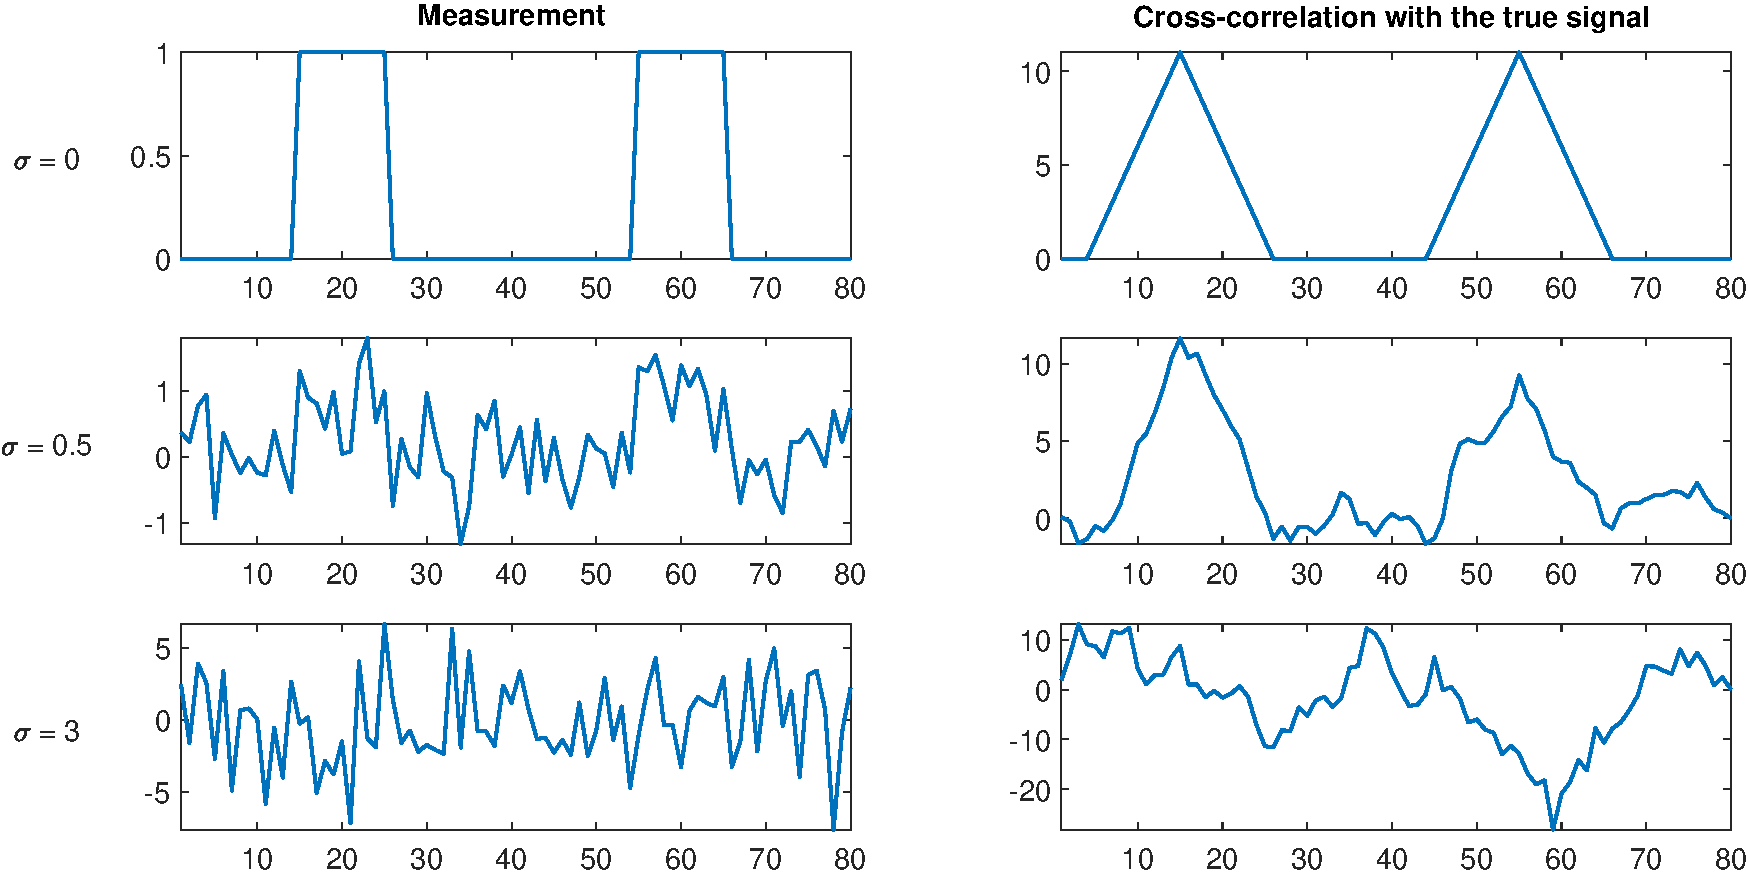
\includegraphics[scale=0.5]{XC_example}
		\caption{ The upper left panel shows a data sequence (measurement) of length $N=80$ with one rectangular signal of length $L=11$ that appears twice. The upper right panel shows the cross-correlation of the data with the true rectangular signal.  
		The second and third rows present the data sequence with additive Gaussian noise with mean zero and standard deviation $\sigma=0.5$ and $\sigma=3$, respectively, and its cross-correlation with the signal. Note to the different scales in different panels. Importantly, in the low $\SNR$ regime the cross-correlation does not provide information on the locations of the signal in the data.}
    	\label{fig:XC_example}
\end{figure}




%
%This work is primely motivated by cryo-electron microscopy (cryo--EM), which is an innovative  single particle reconstruction technology. The acquired data in a cryo-EM experiment is contaminated with high noise levels. Therefore, any molecule reconstruction algorithm must take  the challenging $\SNR$ level into account.  In the last part of this manuscript, we draw connections with the estimation problem under consideration and the cryo--EM problem.


\section{Model and related literature}  \label{sec:model}

Let $x_1,\ldots,x_K\in\RL$ be the sought signals and let $y\in\RN$ be the data. 
A plain way to present the forward model is as a mixture of blind deconvolution problems between binary signals and the target signals
\begin{equation} \label{eq:model}
y = \sum_{i=1}^K x_i\ast s_i + \varepsilon,\quad \varepsilon\sim\mathcal{N}(0,\sigma^2 I).
\end{equation}
%We model the background information as i.i.d.\ Gaussian noise with zero mean and $\sigma^2$ variance. 
Each  $s_i\in\{0,1\}^N$ is associated with the position of the occurrences of the corresponding $x_i$. Let $\mathcal{S}_i$ denotes the set of  the nonzero
 values of $x_i$ and assume that the all $\mathcal{S}_i$'s are disjoint. The union of supports is denoted by $s = \sum_{i=1}^Ks_i$ and similarly $\mathcal{S} = \cup \mathcal{S}_i$. 
The cardinality of the sets are denoted by $\vert \mathcal{S}_i\vert = M_i$ and $\vert \mathcal{S}\vert :=M =  \sum_{i=1}^{K}M_i$.  Neither the $M_i$'s nor $M$ are assumed to be known. 

In order to estimate the mixture of signals autocorrelations, we assume that the support of $s$ is not clustered. In particular, 
\begin{equation} \label{eq:spacing}
\text{For all }  i,j\in\mathcal{S}, \, i\neq j,  \quad  \vert i-j \vert\geq L-1.  
\end{equation}
The goal of the problme is to estimate $x_1,\ldots,x_K$ from $y$.

Blind deconvolution is a longstanding problem, arising in a variety of engineering and scientific applications, such as astronomy, communication, image deblurring, system identification and optics; see~\cite{jefferies1993restoration,shalvi1990new,ayers1988iterative,abed1997blind}, just to name a few. 
To make the problem well-posed, we must  assume some prior knowledge or  structure. 
In our case, the prior information is that $s$ is a binary signal that satisfies~\eqref{eq:spacing}. 
Other settings of blind deconvolution problems have been analyzed recently, see for instance~\cite{ahmed2014blind,li2016identifiability,li2016rapid,ling2015self,ling2017blind,chi2016guaranteed}
where the focus is on high $\SNR$ regimes.


An important feature of the problem under consideration is that while both $x_i$'s and $s_i$'s are unknown, the goal is merely to estimate the $x_i$'s. The  $s_i$'s  are referred to as \emph{nuisance  variables}. Indeed, in many blind deconvolution applications the sole purpose is to estimate one of the unknown signals. For instance, in image deblurring, both the blurring
kernel and the high-resolution image are unknown, but the primary goal is only
to sharpen the image.

If $x$ is known and $K=1$, then a sparse signal can be estimated by linear programming  in the high $\SNR$ regime, e.g.,~\cite{de2012exact,duval2015exact,bendory2016robust,bendory2017robust,bernstein2017deconvolution}. However, in the low $\SNR$ regime, estimating $s$ is impossible. To see that, suppose that an oracle provides us $M$ windows of length $W>L$, each contains one copy of $x$. That is to say, we get a series of windows, each one contains a signal at unknown location. 
Estimating the position of the known signal within each  window is an easier problem than detecting the support of $s$. 
However, even this problem is impossible in the low $\SNR$ regime~\cite{aguerrebere2016fundamental}. Therefore, we conclude that detecting the nonzero values of $s$ is impossible in low $\SNR$. As aforementioned, this work focuses on this regime and examines under what conditions we can estimate the signals themselves, despite the impossibility of detecting their individual occurrences.

For $K=1$, our problem can be also interpreted as a special case of the system identification problem. Similarly to~\eqref{eq:model}, the system identification forward model takes the form
\begin{eqnarray}
y = x\ast w + \varepsilon,  
\end{eqnarray} 
where $x$ is the unknown signal (``system''), $w$ is an unknown, random, input sequence and $\varepsilon$ is an additive noise.   
%The problem has also been studied in the case of a known input $w$~\cite{pillonetto2010new,dinuzzo2015kernels,bottegal2016robust}. 
The goal of this problem is to estimate $x$ (identify the system). The question of identifiability of $x$ under
this observation model is addressed for certain Gaussian and non-Gaussian $w$ in~\cite{benveniste1980robust,kormylo1983identifiability}.
In the special case where $w\in\{0,1\}^N$, satisfying the spacing requirement~\eqref{eq:spacing}, we obtain our
model in the  case of a single signal ($K = 1$).

Likelihood-based methods seek to maximize the likelihood function for $x$,
given the observed signal $y$. Solving this optimization exactly is typically
intractable, and so heuristic methods are used instead. One proposed heuristic
 is to use Markov Chain Monte Carlo (MCMC); in special
cases, including the case where $w$ is binary, EM has been used~\cite{cappe1999simulation}.
The EM method is based upon a certain ``forward-backward'' procedure
used in hidden Markov models, described in~\cite{rabiner1989tutorial}. \TODO{We need to explain}
Other problems solve for parameterized models of $x$; for instance, see~\cite{andrieu2001bayesian}. 
That same paper also considers multiple distinct signals $x$, as in our heterogeneity framework ($K>1$). Their proposed
solution is an MCMC algorithm designed for their specific parametrized problem.

Because likelihood methods are computationally expensive, methods based
on recovery from moments and cumulants, which are akin to our method, have
also been previously used for system identification. The question of identifiability
of $x$ from third-order statistics with non-Gaussian $w$ was considered in~\cite{lii1982deconvolution}. \TODO{how is it different from bispectrum inversion?}
Methods using the third- and fourth-order cumulants are described in~\cite{giannakis1989identification,tugnait1984identification}.


\section{Autocorrelation analysis}   \label{sec:autocorrelation}

Our method for estimating the signals is a two-stage technique. 
First, we use the autocorrelation functions of the data to estimate a mixture (i.e., linear combination) of the $K$ signal's autocorrelations. The mixed autocorrelation can be estimated to any accuracy, in any $\SNR$ level, if $M$ is large enough and the spacing condition~\eqref{eq:spacing} is met. Then, we  use a nonconvex LS  to estimate the signals from their mixed autocorrelations. 
In this section we elaborate on the autocorrelation functions and their estimations, while the precise recovery procedure, based on nonconvex optimization, will be discussed in detail in the next section.


\subsection{Aperiodic autocorrelation functions} \label{sec:aperiodic_ac}

For the purpose of this paper, we need the first three (aperiodic) autocorrelation functions. The first-order autocorelation is the mean of the signals. For  
$z\in\RL$ and $k\geq 2$, the autocorrelation of order $k$ is defined for any integer shifts $\ell_1, \ldots, \ell_{k-1}$ by
\begin{align}
	a_z^k[\ell_1,\ldots,\ell_{k-1}]  & = \sum_{i=-\infty}^{+\infty} z[i]z[i+\ell_1]\ldots z[i+\ell_{k-1}],
	\label{eq:ac_general}
\end{align}
where indexing of $z$ out of the bounds $0, \ldots, L-1$ is zero-padded, as usual.
Explicitly, the first three autocorrelations are
\begin{align} 
	a_z^1 & = \sum_{i=0}^{L-1} z[i], \nonumber\\
	a_z^2[\ell] & = \sum_{i = \max\{0, -\ell\}}^{L-1 + \min\{0, -\ell\}} z[i]z[i+\ell], \nonumber\\
	a_z^3[\ell_1,\ell_2] & = \sum_{i = \max\{0, -\ell_1, -\ell_2\}}^{L-1 + \min\{0, -\ell_1, -\ell_2\}} z[i]z[i+\ell_1]z[i+\ell_2]. \label{eq:ac_special}
\end{align}
Note that the autocorrelation functions are symmetric so that $a_z^2[\ell] = a_z^2[-\ell]$ and $a_z^3[\ell_1,\ell_2] = a_z^3[-\ell_1,-\ell_2]$. \TODO{We also have $a_z^3[\ell_1,\ell_2] = a_z^3[\ell_2,\ell_1]$ -- is that intended? Do we really have symmetry with the negative signs? I think we have $(\ell_1, \ell_2) \sim (-\ell_1, \ell_2-\ell_1)$; to be checked, but I don't think this is correct;}
Additionally, if the moments of the signal depend only on the difference between the indices (Toeplitz structure), then they are equivalent to the autocorrelation functions.

A one-dimensional signal is determined uniquely and stably by its third-order auto-correlation as proven in the following simple proposition.
\begin{proposition} \label{prop:uniqueness}
	Let $z\in\RL$ and suppose that $z[0]$ and $z[L-1]$ are nonzero. Then:
	\begin{itemize}
		\item \textbf{Uniqueness:} 	 $z$  is determined uniquely from  $a_z^2$ and $a_z^3$.
        \item \textbf{Finite sensitivity:} 	Suppose that  $a_z^3[k,L-1]$ can be estimated up to  perturbation $\upsilon$ and let $\hat{z}[k]$ be an estimator of $z[k]$. If $\vert z[0]z[L-1]\vert \geq \delta>0$, then $\vert \hat{z}[k] - z[k]\vert\leq \frac{\vert \upsilon\vert }{\delta}$. \TODO{That statement is incomplete: you mean there exists an estimator that guarantees this. (Since the estimator is very simple, we may want to show it explicitly in the proposition statement, and comment afterwards that of course this is still fairly sensitive, and we can do better.)}
	\end{itemize}
	\begin{proof}
		By assumption $a_z^2[L-1] = z[0]z[L-1]\neq 0$.
		Then, the uniqueness results, for all $k=0,\ldots L-1$,  follows from:
		\begin{equation*}
		a_z^3[k,L-1] = z[0]z[k]z[L-1].
		\end{equation*}
		If we measure $\tilde{a_z^3}[k,L-1] = a_z^3[k,L-1]+\upsilon$, then 
		\begin{equation*}
		\hat{z}[k] = \frac{\tilde{a_z^3}[k,L-1]}{a_z^2[L-1]} = z[k]+\frac{\upsilon}{a_z^2[L-1]} \quad \Rightarrow \quad \vert \hat{z}[k] - {z}[k]\vert \leq \frac{\vert\upsilon\vert}{\delta}.
		\end{equation*} 
	\end{proof}
\end{proposition}

A few remarks are in order. First, this result carries through to signals of any dimension.
Second, if the spacing condition~\eqref{eq:spacing} holds, then the length of the signal can be determined from the autocorrelations and 
therefore the assumption that the first and last entries are nonzero is met. In particular, if~\eqref{eq:spacing} holds for some spacing $W>L$, then $a_z^2[i]=0$ for all $i>L-1$.
Third, computing the $d$th autocorrelation amplifies the variance of the noise by a factor $d$ asymptotically. Therefore, if we can estimate $a_z^3$ up to small perturbation, it implies that we can estimate $a_z^2$ accurately as the proposition assumes. 
Finally, while Proposition~\ref{prop:uniqueness} shows only finite sensitivity, in practice LS estimator is robust to additive noise; see Section~\ref{sec:numerics}. This is compatible with results in related problems~\cite{bendory2017bispectrum,boumal2017heterogeneous}.

Considering the third-order autocorrelation is also a necessary condition to determine a signal from its autocorrelations. Indeed, the second-order autocorrelation of a one-dimensional signal does not determine a signals uniquely~\cite{beinert2015ambiguities,bendory2017fourier}. On the other hand, for dimensions greater than one, almost all signals are determined uniquely, up to sign (phase in the complex case) and reflection through the origin (with conjugation in the complex case)~\cite{hayes1982reconstruction,hayes1982reducible}. The sign ambiguity can be resolved by the mean of the signal if it is not zero. However,  in order to determine the reflection symmetry, one needs to use additional information.

\TODO{I would remove most if this paragraph; we can have a similar discussion but for our case (after having discussing which moments we keep); make the statement, and finish with a one-sentence reference to the MRA paper.}
The invertibility of the autocorrelations for $K>1$ was explored  for the related case of  periodic autocorrelation functions. Recall that the  periodic autocorrelations are defined similarly to~\eqref{eq:ac_general}, with two differences: the sum goes to $L-1$ and all indices should be taken modulo $L$.
If $z[n]=0$ for $n=L/2,\ldots L-1$ (``zero-padded''), then the periodic and aperiodic autocorrelation coincide.
In~\cite{bandeira2017estimation}, it was shown that a mix of $K$ third-order periodic autocorrelations determine  a finite list of $K$ generic signals if $L/6\gtrsim K$. Empirical evidences hints that this finite list includes only group symmetries, at least as long as $K\leq\sqrt{L}$~\cite{boumal2017heterogeneous}. 


\subsection{Estimating autocorrelations from the data with a single signal $K=1$} \label{sec:estimating_ac_k1}

We first consider the problem of estimating the autocorrelations of a single signal from the data. 
All the main concepts carry through for $K>1$ as will be shown in the next section.  

In order to estimate the autocorrelations of the signal, we first compute the first $L$ entries of the data's autocorrelations. 
For the purpose of the analysis, we consider  the asymptotic regime where $M,N\to\infty$, while preserving fixed ratio. 
Specifically, we define the ratio of the measurement occupied by  the signal as
\begin{equation}
\gamma = \frac{M L}{N}.
\end{equation}
Under the spacing constraint~\eqref{eq:spacing}, we have $\gamma\leq\frac{L}{2L-1}\approx 1/2$.

The main pillar of this work is the following simple observation.
If the support $s$ satisfies the spacing constraint~\eqref{eq:spacing}, then the first $L$ entries of the data autocorrelations converge 
to a scaled, biased, version of the signal's autocorrelation:
\begin{align}
\lim_{N\to\infty} a_y^1 & = \gamma a_{x}^1, \nonumber\\
\lim_{N\to\infty} a_y^2[\ell] & = \gamma a_{x}^2[\ell] +\sigma^2\delta[\ell], \label{eq:data_ac_k1} \\
\lim_{N\to\infty} a_y^3[\ell_1,\ell_2] & = \gamma a_{x}^3[\ell_1,\ell_2] + \sigma^2\gamma a_{x}^1 \big(\delta[\ell_1,0]+\delta[0,\ell_2]+\delta[\ell_1,\ell_2]\big), \nonumber
\end{align}
for $\ell,\ell_1,\ell_2=0,\ldots L-1$, and where $\delta$ denotes the Kronecker delta function. 
These relations are proven in Appendix~\ref{sec:autocorrelation_computation}. The analysis is similar to~\cite{bendory2017bispectrum,boumal2017heterogeneous}, yet a particular caution should be taken with the statistical dependencies of the noise entries. 
The relations~\eqref{eq:data_ac_k1}, together with Proposition~\ref{prop:uniqueness}, imply that given $M$ and $\sigma$, one can estimate the signal for any noise level if $M$ is large enough. Next, we show that  $M$ and $\sigma$ are also uniquely determined from the autocorrelations. 

If the noise level $\sigma^2$ is known, one can estimate the ratio $M/N$ from the first two moments.
\begin{proposition} \label{prop:gamma}
	Let $K=1$, $N\to\infty$ and $\sigma$ fixed. If the mean of $x$ is nonzero, then 
	\begin{equation*}
	\frac{M}{N} = \frac{1}{L}\frac{(a^1_y)^2}{\sum_{j=0}^{L-1}a_y^2[j]-\sigma^2}.
	\end{equation*}
	\begin{proof}
The proof follows from plugging the explicit expressions of~\eqref{eq:data_ac_k1} into the right hand side of the equality.
\end{proof}
\end{proposition}

If we use third-order autocorrelation information, then it is possible to estimate both the ratio $M/N$ and $\sigma$ simultaneously.
\begin{proposition} \label{prop:gamma_sigma}
	Let $K=1$, $N\to\infty$ and $\sigma$ fixed. Then, $a_y^1,a_y^2$ and  $a_y^3$ determine the ratio $M/N$ and $\sigma$ uniquely for generic signals. If $\frac{M}{N}\geq\frac{1}{4(L-1)}$, then it holds for any signal with nonzero mean. 
	\begin{proof}
		See Appendix~\ref{sec:proof_prop_gamma_sigma}.
	\end{proof}
\end{proposition}

From Propositions~\ref{prop:uniqueness} and~\ref{prop:gamma_sigma} we can directly deduce the following.
\begin{corollary}
	Let $K=1$, $N\to\infty$ and $\sigma$ is fixed. Then, the signal, the ratio $M/N$ and $\sigma$ can be recovered from the first three autocorrelation functions if:
	\begin{itemize}
		\item $x$ is generic;
		\item  $x[0],x[L-1]\neq 0$, $x$ has nonzero mean and $\frac{M}{N}\geq\frac{1}{4(L-1)}$.
	\end{itemize}
\end{corollary}
 
 
\subsection{Estimating autocorrelations from the data with multiple signals $K>1$} \label{sec:estimating_ac}

When $K>1$, it is impossible \TODO{That's not true: we can do our procedure, which gives estimate of the signals, and moments of that are estimates of the moments of the individual signals. Whether one calls this 'direct' or not is subjective. I'd remove that sentence.)} to estimate the autocorrelation of each signal directly from the data. However similarly to~\eqref{eq:data_ac_k1}, one can estimate the mixture of the autocorrelations. 
As before, we consider  the asymptomatic regime where $M_1,\ldots,M_K,N\to\infty$, while preserving fixed ratios
\begin{align}
	\gamma_k = \frac{M_k L}{N}, \quad \gamma = \sum_{k=1}^K\gamma_k.
\end{align}
If the support $s$ satisfies the spacing constraint~\eqref{eq:spacing}, then:
\begin{align}
\lim_{N\to\infty} a_y^1 & = \sum_{k=1}^K\gamma_k a_{x_k}^1, \nonumber\\
\lim_{N\to\infty} a_y^2[\ell] & = \sum_{k=1}^K\gamma_k a_{x_k}^2[\ell] +\sigma^2\delta[\ell],  \label{eq:data_ac}\\
\lim_{N\to\infty} a_y^3[\ell_1,\ell_2] & = \sum_{k=1}^K\gamma_k a_{x_k}^3[\ell_1,\ell_2] + \sigma^2\left(\sum_{k=1}^K\gamma_k a_{x_k}^1\right)(\delta[\ell_1,0]+\delta[0,\ell_2]+\delta[\ell_1,\ell_2]), \nonumber
\end{align}
This relation is proven in  Appendix~\ref{sec:autocorrelation_computation}.

The minimal order of data statistics used to get an accurate estimation of a signal is important to understand, in the asymptotic $\SNR$ regime, the sample complexity of the problem.
In methods which are based on detection and averaging, the number of signals occurrences  must scale like $\sigma^2$. Taking the $d$th order autocorrelation function amplifies the variance of the noise by a factor of $d$. Therefore, the required number signal occurrences should scale like $\sigma^{2d}$  to retain some constant estimation error. Accordingly, in our  method, $M$ must scale like $\sigma^6$. In Section~\ref{sec:numerics}, we show empirically the third-order autocorrelation suffices also for a mixture of $K>1$ signals without prior knowledge of the $M_i$'s and $\sigma$.  \TODO{question mark on the entire paragraph}
\TODO{We could move here the paragraphs from 1D XP about which moments we compute, to argue that we can expect to recover at most up to $K = L/2$ signals.}


\section{Numerical experiments}   \label{sec:numerics}

%\TODO{Here we should say that we can afford to work only with non-biased terms}


%\subsection{One-dimensional experiments}

\TODO{Revise to explain $K = 1$ experiment first, then explain $K = 3$.}

\begin{figure}[t]
	\centering
	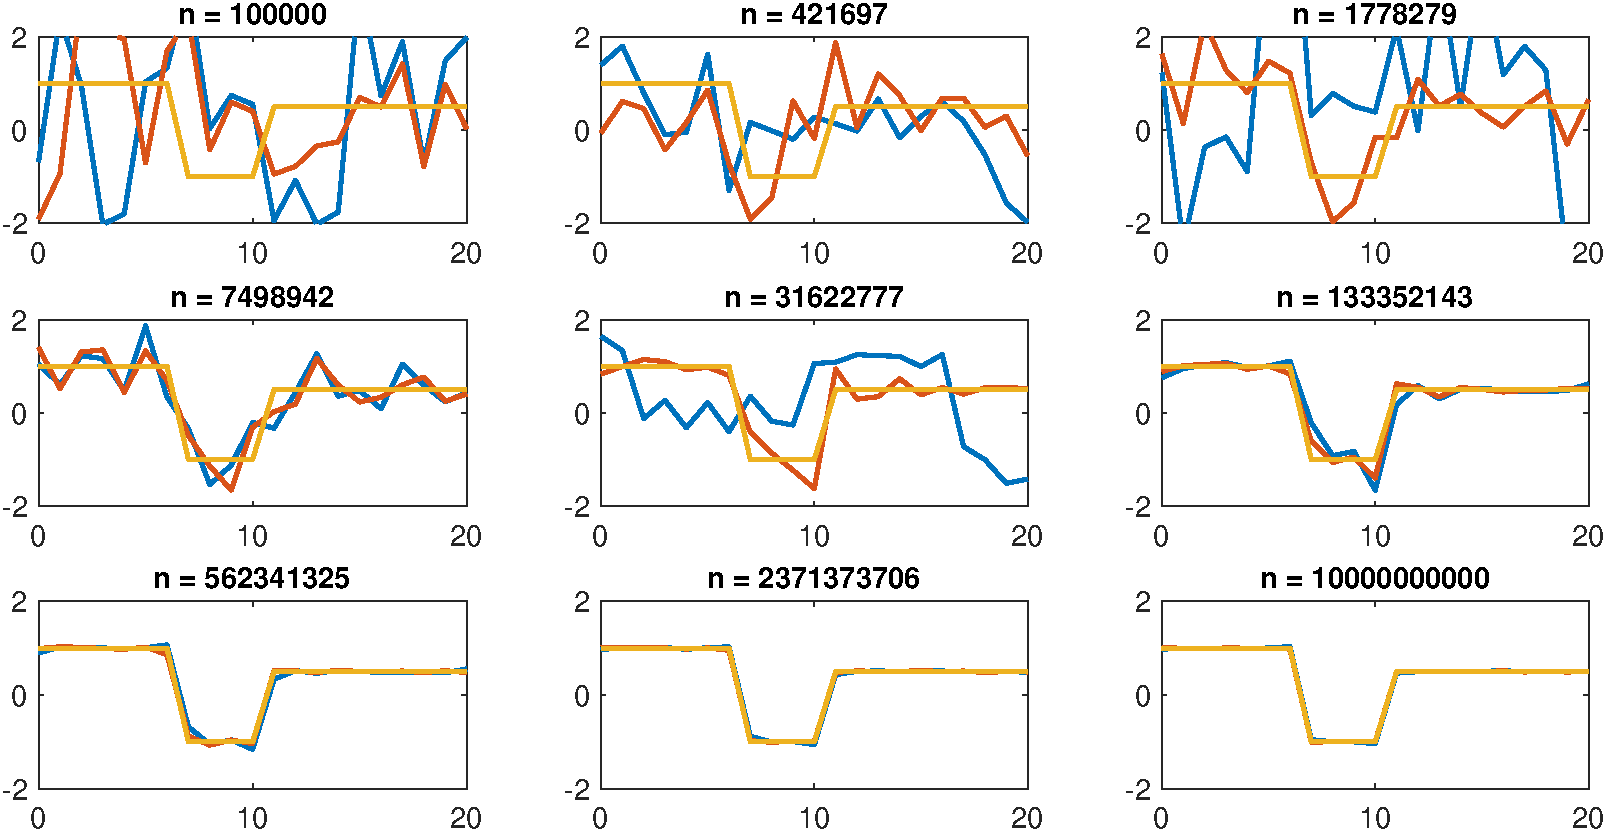
\includegraphics[width=0.7\linewidth]{XP_1D_homogeneous/progressive_n10000000000_107521}
	\caption{\TODO{...}}
	\label{fig:1Dhomosignals}
\end{figure}

\begin{figure}[t]
	\centering
	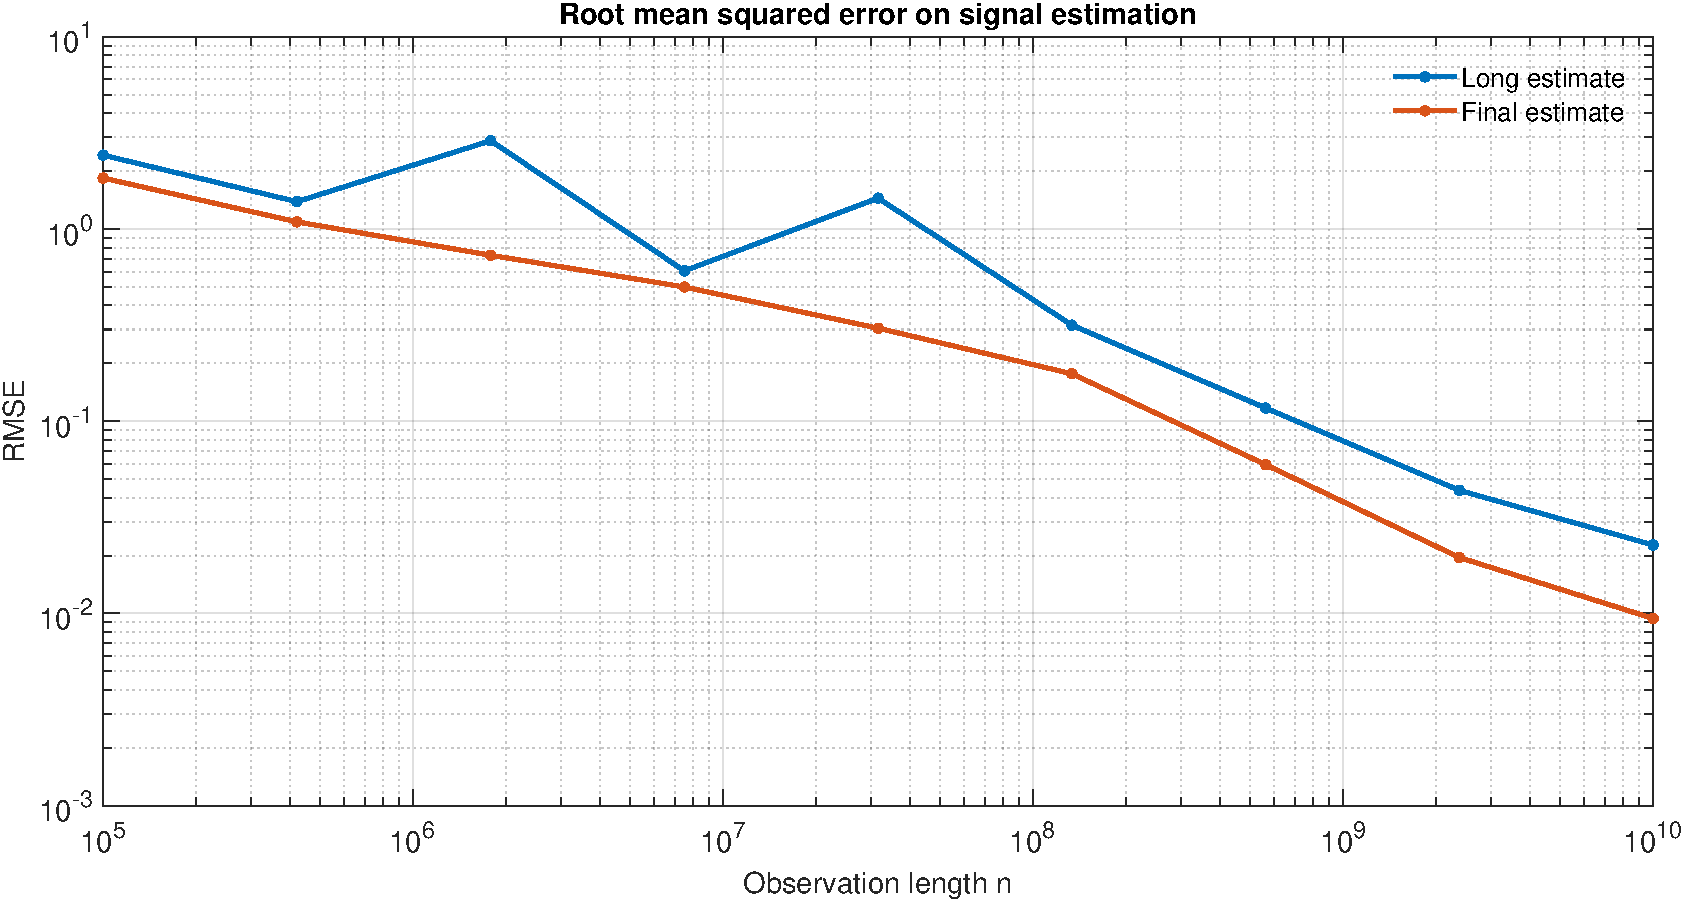
\includegraphics[width=0.7\linewidth]{XP_1D_homogeneous/progressive_RMSE_n10000000000_107521}
	\caption{\TODO{...}}
	\label{fig:1DhomoRMSE}
\end{figure}


For the 1D experiment, we fix $K = 3$ signals of length $L = 21$, as depicted in Figure~\TODO{ref}. Following the data model described in Section~\TODO{ref}, we generate an observation $y$ of length $24.6 \cdot 10^9$. Each of the three signals appears, respectively (and approximately) $300 \cdot 10^6$, $200 \cdot 10^6$ and $100 \cdot 10^6$ times in $y$, such that at least $L-1$ zeros separate two occurrences of any signals. This is done by randomly selecting $600 \cdot 10^6$ placements in $y$, one at a time with an accept/reject rule based on the separation constraint and locations picked so far. For each placement, one of the three signals is picked at random proportionally to the desired number of occurrences of each. Then, i.i.d.\ Gaussian noise with mean zero and standard deviation $\sigma = 3$ is added, to form the observed $y$. The SNR of $y$
% sqrt((m_want*sum(X.^2)')/(sigma^2*n))
is about 1/12.
%Given the scaling of the target signals (whose median absolute value for the entries is at or below one),
This is enough noise to make cross-correlations of $y$ even with the true signals display peaks at random locations, uninformative of the actual locations of the signal occurrences. Thus, we contend that it would be difficult for any algorithm to locate the signal occurrences, let alone to classify them according to which signal appears where.

Given the observation $y$, we proceed to compute the moments. The first-order moment is straightforward. For second-order moments, notice from equation~\eqref{eq:data_ac} that $a_y^2[\ell]$ suffers no bias for $\ell$ in $1$ to $L-1$. Thus, we omit $\ell = 0$, which has the practical effect that we need not know $\sigma$ to estimate the moments. Likewise, for third-order moments, $a_y^3[\ell_1, \ell_2]$ for $0 \leq \ell_1, \ell_2 \leq L-1$ such that $\ell_2 \leq \ell_1$ includes all relevant moments for our purpose \TODO{Do we want to include a figure to explain why that is?}, and we further exclude any such that $\ell_1, \ell_2$ or $\ell_1 - \ell_2$ are zero to avoid biased elements---there are $\frac{(L-1)(L-2)}{2}$ remaining moments. As a result, it is unnecessary to estimate $\sigma$. We have
\begin{align*}
	1 + (L-1) + \frac{(L-1)(L-2)}{2} = \frac{1}{2} L (L-1) + 1
\end{align*}
moments in total. In practice, these are computed on disjoint segments of $y$ of length $100\cdot10^6$ and added up, without correction for the junction points. Segments are handled sequentially on a GPU, as GPUs are particularly well suited to execute simple instructions across large vectors of data. If multiple GPUs are available, segments can of course be handled in parallel.

Having computed the moments of interest, we now estimate signals $x_1, \ldots, x_K$ and coefficients $\gamma_1, \ldots, \gamma_K$ which agree with the data. We choose to do so by running an optimization algorithm on the following nonlinear least-squares problem:
\begin{multline}
	\min_{\substack{\hat x_1, \ldots, \hat x_K \in \reals^{W} \\ \hat \gamma_1, \ldots, \hat \gamma_K > 0}} w_1 \left( a_y^1 - \sum_{k=1}^K \hat \gamma_k a_{\hat x_k}^1 \right)^2 + w_2 \sum_{\ell = 1}^{L-1} \left( a_y^2[\ell] - \sum_{k=1}^K \hat \gamma_k a_{\hat x_k}^2[\ell] \right)^2 + \\ w_3 \sum_{\substack{2\leq\ell_1\leq L-1 \\ 1 \leq \ell_2 \leq \ell_1-1}} \left( a_y^3[\ell_1, \ell_2] - \sum_{k=1}^K \hat \gamma_k a_{\hat x_k}^3[\ell_1,\ell_2] \right)^2.
	\label{eq:optim1D}
\end{multline}
where $W \geq L$ is the length of the sought signals and \TODO{explain $w_i$'s: currently they are $w_1 = 1/2, w_2 = 1/2n_2, w_3 = 1/2n_3$, where $n_2, n_3$ are the number of moments used: $n_2 = L-1$, $n_3 = \frac{(L-1)(L-2)}{2}$. Issue is: this is not very smart..}. Setting $W = L$ (as is a priori desired) is problematic because the above optimization problems appears to have numerous poor local optimizers.
%Since we can only initialize randomly at first, this approach would often fail in practice. Alternatively,
Thus, we first run the optimization with $W = 2L-1$. This problem appears to have fewer poor local optima, perhaps because the additional degrees of freedom allow for more escape directions. Since we hope the signals estimated this way correspond to the true signals zero-padded to length $W$, we extract from each one a subsignal of length $L$ (with cyclic indexing \TODO{we should understand / explain this}) that has largest $\ell_2$-norm. This estimator is then used as initial iterate for~\eqref{eq:optim1D}, this time with $W = L$. We find that this procedure is reliable for a wide range of experimental parameters. To solve~\eqref{eq:optim1D}, we run the trust-region method implemented in Manopt~\cite{manopt}, which allows to treat the positivity constraints \TODO{I might need a reference for this} on coefficients $\hat \gamma_k$. Notice that the cost function is a polynomial in the variables, so that it is straightforward to compute it and its derivatives.
\TODO{Should we do variable projection for the gammas, that is, exploit the fact the problem is a regular least squares in the gammas (up to the positivity constraints) to substitute the explicit optimum for them? Not sure it's worth the effort. -- Ok, it's probably not a good idea, because even with fixed gammas to the correct value, optimization takes a while.}
\TODO{Do we still need to stress at this point that the optimization part has complexity independent of length of observation? Should be pretty clear at this point already.}

%\subsection{Two-dimensional experiments} 
%?? 

%
%In this section, we provide the details of the 2D experiment shown in Figure~\ref{fig:example}. In the experiment, we generated a sequence of $767\times 10^3$ 2D images (``micrograph") of size $2000\times 2000$. Each micrograph had around $\sim 900$ signal occurrences (depends on the stopping criterion that we need to explain) and in total $M = 561\times 10^6$. The noise level was $\sigma=1$.  
%
%To accelerate the experiment, we estimated only the first two autocorrelations of the signal. As mentioned in Section~\ref{sec:estimating_ac}, this data determines a 2D signal uniquely, up to possible reflection symmetry. 
%In this experiment, we chose the correct reflection manually. To estimate the signal we used the Relax-Reflect-Reflect (RRR) algorithm, which is a known phase retrieval algorithm. Recall that the second-order autocorrelation is equivalent to the power spectrum of the signal.
%Starting form random initialization of size $(2L-1)\times(2L-1)$, its $k$th  iteration take the form of 
% \begin{equation*}
% x_k = x_{k-1} + \beta(P_2(2P_1(x_{k-1}) -x_{k-1}) - P_1(x_{k-1}), 
%  \end{equation*}
% where $P_1$ is a projection that keeps the values of the  $L\times L$ entries in the upper-left corner and zeros out all other entries, $P_2$ is a projection that keeps the Fourier phase of $x_{k-1}$ and impose the correct Fourier magnitudes, and we set $\beta = 0.5$. The solution of the RRR scheme was used to initialized a LS estimation on the first two moments with signals of length $(2L-1)\times(2L-1)$ for the 200 iterations. Finally, we chose the $L\times L$ upper left corner and refined it using LS with 500 iterations. 
% 

\section{Open questions}

In this paper, we considered the problem of estimating a set of signals from their multiple occurrences in unknown locations in the data.  We focused on  low $\SNR$ environments in which detection is impossible. 
Our technique  is based on computing the third-order autocorrelation function of the data with asymptotic estimation rate proportional to $\sigma^6/M$. Based on related results in multireference alignment~\cite{abbe2018estimation}, we believe that it is the optimal estimation rate, however, this is yet to be proven.

Our results rely on two main assumptions that are not necessarily met by applications. 
First, we modeled the background information as i.i.d.\ additive noise. In practice,
the background information may be structured, and even signal-dependent. Then, the question is  under what conditions  
one can still estimate the signals and separate them from the background information in the low $\SNR$ regime? 

In addition, we assumed that the signal occurrences are all separated by $L-1$ entries, see~\eqref{eq:spacing}. If the signals are not separated, one can introduce a new variable $p$ that represents the distribution of the spacing between signal occurrences. The first entry $p[1]$ will represent the probability that two consecutive signals are separated by only one entry, $p[2]$ the probability for spacing of two entries and so on. Using this new variable $p$, one can write explicitly the relation between the autocorrelation functions of the data and those of the signal in a similar way to~\eqref{eq:data_ac}. Under what conditions on $p$ and the signals one can still estimate the signals from the data?


\section{Connection with the cryo--EM problem}	

Cryo--EM is an innovative technology for reconstructing the 3D structure of macromolecules. In recent years, structures
of many molecules, previously regarded as insurmountable, are now being
obtained to near-atomic resolution; see for instance~\cite{kuhlbrandt2014resolution,bartesaghi20152}. This technological advancement was recognized by the 2017 Nobel Prize in Chemistry~\cite{nobel}. 

In a cryo--EM experiment, multiple biological samples of the (ideally) same molecule are rapidly frozen in a thin layer of vitreous ice. Within the ice, the molecules are randomly oriented and positioned. Then,  the microscope produces a 2D tomographic projection image, called a \emph{micrograph}, of the multiple samples embedded in the ice. Importantly, the micrograph is dominated by noise due to the small electron doses that
can be applied to the specimen without causing radiation damage.

The cryo--EM problem is to estimate the structure of the molecule from the micrograph (or, typically, several micrographs). 
All contemporary methods in the field split the reconstruction procedure to several subroutines. 
The first step in the pipeline is the so called particle picking, in which one aims to detect the 2D tomographic projections of the samples from the noisy micrograph. The output of ideal particle picker is a series of 2D images, each contains one centered tomographic projection associated with unknown 3D orientation. This series of images 
 is then used by a variety of algorithms to reconstruct the structure. 
However, due to the high noise level, the performance of particle pickers  is not ideal. For instance, the projections in the 2D images are typically not centered, increasing dramatically the number of parameters involved in the estimation problem. In addition, the information from particles that are too close to each other is usually neglected. Hence, valuable information that can be used is omitted. 

The model considered in this paper can be interpreted as a preliminary step towards investigation of the possibility to \emph{estimate the molecule's structure directly from the micrograph}. 
In our model, the noisy data $y$ is the analog of the micrograph. The $K$ sought signals correspond to $K$ different molecule's projections, each taken from  different unknown viewing direction. %In tomography, if enough projections are estimated, then one can estimate the whole structure (up to some $K$-dependent resolution).
The position of individual projections are the nuisance variables of the cryo--EM problem (as well as the viewing directions), in analogy to individual signal's locations in our setup.
That being said, the cryo--EM data is far more complicated that the simplified model of this paper. In a future research, we hope to bridge this gap.
 
%For instance, the numerical experiments of Section~\ref{sec:numerics} indicate that we need a huge number of observations to obtain an accurate estimate. Can we accelerate the estimation rate? How to include nearby molecule to extract all information in the micrograph?
%In addition, since the size of a micrograph is quite large (typically around $4000\times 4000$ pixels), computing the third-order autocorrelations may be  expensive if not implemented carefully by parallelizing the computations.
%

\bibliographystyle{plain}
\bibliography{ref}



\appendix

\section{Autocorrelation estimations} \label{sec:autocorrelation_computation}

Throughout the proof, we consider the case of one signal $K=1$. The extension to $K>1$ is straightforward by averaging the contributions of all signal with  appropriates weights, see~\cite{boumal2017heterogeneous}. 

Let us define
\begin{equation}
\gamma = \lim_{N\to\infty} \frac{M_NL}{N}<1.
\end{equation}
With a bit abuse of notation, $M_N$ stresses that $M$ is a function of $N$. Indeed, by assuming $M_N=\Omega(N)$, we deduce $\gamma>0$.
We start by considering the first autocorrelation of the data
\begin{equation}
a_y^1 = \sum_{i=0}^{N-1} y[i] = \frac{1}{N/L}\sum_{j=0}^{M_N-1}\frac{1}{L}\sum_{i=0}^{L-1}x[i] + \underbrace{\frac{1}{N}\sum_{i=0}^{N-1}\varepsilon[i]}_{\text{noise term}} \xrightarrow{a.s.}\gamma a_x^1,
\end{equation}
where the noise term converges to zero almost surely (a.s.) by the law of large numbers.

We proceed with the second autocorrelation for fixed $\ell\in[0,\ldots,L-1]$. We can compute:
\begin{equation}
\begin{split}
a_y^2[\ell] & = \frac{1}{N}\sum_{i=0}^{N-1-\ell}y[i]y[i+\ell] \\
& \underbrace{\frac{1}{N}\sum_{j=1}^{M_N}\sum_{i=0}^{L-\ell-1}x[i]x[i+\ell]}_{\text{signal term}} + \underbrace{\frac{1}{N}\sum_{i=0}^{N-1-\ell}\varepsilon[i]\varepsilon[i+\ell]}_{\text{noise term}},
\end{split}
\end{equation}
where the cross terms between the signal and the noise vanish  almost surely in the limit $N\to\infty$. 

We treat the signal and noise terms separately. We first break the signal term into $M_N$ different sums, each contains one copy of the signal, and get
\begin{equation} \label{eq:2nd_moment_signal_term}
\frac{1}{N}\sum_{j=1}^{M_N}\sum_{i=0}^{L-\ell-1}x[i]x[i+\ell] = \frac{M_NL}{N}\frac{1}{L}\sum_{i=0}^{L-\ell-1}x[i]x[i+\ell] = \gamma a_x^2[\ell].
\end{equation}
Similarly, for $\ell\neq 0$, we can break the noise term into a sum of independent terms 
\begin{equation}
\frac{1}{N}\sum_{i=0}^{N-1-\ell} \varepsilon[i]\varepsilon[i+\ell] = \frac{1}{\ell}\sum_{i=0}^{\ell-1}\frac{1}{N/\ell}\sum_{j=0}^{N/\ell -1} \varepsilon[j\ell + i] \varepsilon[(j+1)\ell + i].
\end{equation}
Each term of $\frac{1}{N/\ell}\sum_{j=0}^{N/\ell -1} \varepsilon[j\ell + i] \varepsilon[(j+1)\ell + i]$ is an average of $N/\ell$ independent terms with expectation zero, and thus converges to zero almost surely as $N\to\infty$.
If $\ell=0$, 
\begin{equation}
\frac{1}{N}\sum_{i=0}^{N-1} \varepsilon^2[i] \xrightarrow{a.s.} \sigma^2.
\end{equation}

We are now moving to analyze the third-order autocorrelation. Let us fix $\ell_1\geq\ell_2$ and recall that 
\begin{equation*}
a_y^3[\ell_1,\ell_2] = \sum_{i=0}^{N-1-\ell_1} y[i]y[i+\ell_1]y[i+\ell_2]. 
\end{equation*}
Writing explicitly in terms of signal and noise, the sum can be broken into eight terms. The first contains only signal terms (does not see noise) and converges to $\gamma a_x^3$ from the same reasons as~\eqref{eq:2nd_moment_signal_term}. Three other terms contain the product of two signal entries and one noise term. Since the noise is independent of the signal and has zero mean, these terms go to zero almost surely.

We next analyze the contribution of the term composed of triple products of noise terms. For $\ell_1\neq 0$, this sum can be formulate as follows:
\begin{equation*}
\sum_{i=0}^{N-1-\ell_1} \varepsilon[i]\varepsilon[i+\ell_1]\varepsilon[i+\ell_2] = \frac{1}{\ell_1}\sum_{i=0}^{\ell_1-1}\frac{1}{N/\ell_1}\sum_{j=0}^{N/\ell_1 -1 }\varepsilon[j\ell_1+i]\varepsilon[(j+1)\ell_1+i]\varepsilon[j\ell_1+i+\ell_2].
\end{equation*}
For each fixed $i$, we sum of over $N/\ell_1$ independent variables that goes to zero almost surely. For $\ell_1=\ell_2=0$, we get a some of $N$ independent variables, each one is a triple product of Gaussian variables with zero mean and therefore has zero expectation. 

To complete the analysis, we consider the three terms composed of the product of two noise terms and one signal entry. Most of these terms converge to zero almost surely because of independency between the noise entries. For $\ell_1=0, \ell_2=0$ and $\ell_1=\ell_2$,  a simple computation shows that the sum converges to $\gamma\sigma^2a_x^1$; c.f.~\cite{boumal2017heterogeneous}.



\section{Proof of Proposition~\ref{prop:gamma_sigma}} \label{sec:proof_prop_gamma_sigma}

We aim to prove that one can estimate both $\sigma$ and $\beta = M/N$ from the observed first three moments.
To this end, we construct two quadratic equations of $\beta$ from the observed (measured) quantities, independent of $\sigma$.
Then, we show that these equations are independent and therefore $\beta$ is uniquely defined. 
Given $\beta$, we can estimate $\sigma$ using Proposition~\ref{prop:gamma}.
Throughout the proof, it is important to distinguish between observed and unobserved values. 
to this end, we denote the observed values by $E_i$ or $a_y^1,a_y^2,a_y^3$, while using $F_i$ for functions of the signal's autocorrelations. 


Recall that $a_y^1 = \beta(\one^Tx)$ and  
and $a_y^2[0] = \beta\|x\|^2+\sigma^2$, where $\one\in\RL$ stands for vector of ones. Taking the product:
\begin{equation}\label{eq:E1}
\begin{split}
E_1 &:= a_y^1a_y^2[0] =  (\beta(\one^Tx))(\beta\|x\|^2+\sigma^2) \\
& = \sigma^2a_y^1 + \beta^2F_1,
 \end{split}
\end{equation}
where $F_1 := a_x^3[0,0] + \sum_{j=1}^{L-1}(a_x^3[j,j] + a_x^3[0,j])$. 
The terms of $F_1$ can be also estimated from $a_y^3$, while taking the scaling and bias terms into account:
\begin{equation} \label{eq:E2}
E_2:= \beta F_1 + (2L+1)\sigma^2a_y^1.
\end{equation}
Therefore, from~\eqref{eq:E1} and~\eqref{eq:E2} we get
\begin{equation} \label{eq:E12}
E_2\beta -(2L+1)\sigma^2\beta a_y^1 = E_1-\sigma^2a_y^1.
\end{equation}
Let $a_y^2:=\sum_{j=0}^{L-1}a_y^2[j]$ and recall from Proposition~\ref{prop:gamma}:
\begin{equation} \label{eq:sigma2}
\sigma^2 = a_y^2 - (a^1_y)^2/(\beta L). 
\end{equation} 
Plugging into~\eqref{eq:E12} and rearranging we get 
\begin{equation} \label{eq:quad1}
\mathcal{A}\beta^2 + \mathcal{B}\beta + \mathcal{C} = 0,
\end{equation}
where 
\begin{align*}
\mathcal{A} &= E_2 - (2L+1)a_y^1a_y^2, \\ 
\mathcal{B} &= -E_1 + \frac{2L+1}{L}(a_y^1)^3 + a_y^1a_y^2  , \\
\mathcal{C} &= -(a_y^1)^3/L.
\end{align*}
Importantly, these coefficients are observable quantities. 

We are now proceeding to derive the second quadratic equation. We notice that 
\begin{equation} \label{eq:E3}
E_3  = \frac{1}{L}(a_y^1)^3 = \frac{1}{L}\beta^3 (\one ^Tx)^3   = \frac{1}{L}\beta^3 F_2,
\end{equation}
where 
\begin{equation*}
F_2 =  a_x^3[0,0] + 3\sum_{j=1}^{L-1}a_x^3[j,j] + 3\sum_{j=1}^{L-1}a_x^3[0,j] + 6\sum_{1\leq i < j\leq L-1}a_x^3[i,j].
\end{equation*}
On the other hand, from $a_y^3$ we can directly estimate $F_2$ up to scale and bias
\begin{equation} \label{eq:E4}
E_4 = \beta F_2 + (6L-3)\sigma^2a_y^1.
\end{equation}
Taking the ratio:
\begin{equation*} 
\frac{E_4}{E_3} = \frac{L}{\beta^2} + \frac{(6L-3)L\sigma^2a_y^1}{E_3}, 
\end{equation*}
we conclude:
\begin{equation*}
\sigma^2 = \frac{E_4}{a_y^1L(6L-3)}  - \frac{E_3}{\beta^2a_y^1(6L-3)}.
\end{equation*}
Using~\eqref{eq:sigma2} and rearranging we get the second quadratic:
\begin{equation} \label{eq:quad2}
\mathcal{D}\beta^2 + \mathcal{E}\beta + \mathcal{F} = 0,
\end{equation}
where
\begin{align*}
\mathcal{D} &= a_y^2 - \frac{E_4}{a_y^1L(6L-3)}, \\ 
\mathcal{E} &= -(a_y^1)^2/L, \\
\mathcal{F} &= \frac{E_3}{a_y^1(6L-3)}.
\end{align*}

To complete the proof, we need to show that the two quadratic equations~\eqref{eq:quad1} and~\eqref{eq:quad2} are independent. To this end, it is enough to show that the ratio between the coefficients is not the same. 
From~\eqref{eq:quad1} and~\eqref{eq:E1}, we have 
\begin{equation*}
\begin{split}
\frac{\mathcal{B}}{\mathcal{C}} &= \frac{LE_1 - (2L+1)(a_y^1)^3 - La_y^1a_y^2}{(a_y^1)^3} \\&= \frac{La_y^2[0] - (2L+1)(a_y^1)^2 - La_y^2}{(a_y^1)^2}.
\end{split}
\end{equation*}
In addition, using~\eqref{eq:E3}
\begin{equation*}
\frac{\mathcal{E}}{\mathcal{F}} = \frac{(3-6L)(a_y^1)^3}{LE_3} = 3 - 6L . 
\end{equation*}

Now, suppose that the quadratics are dependent. Then, $\frac{\mathcal{B}}{\mathcal{C}} =\frac{\mathcal{E}}{\mathcal{F}} $, or, 	
\begin{equation*}
La_y^2[0] - (2L+1)(a_y^1)^2 - La_y^2 = (a_y^1)^2(3-6L)
\end{equation*}
Rearranging the equation and writing in terms of $x$ we get 
\begin{equation} \label{eq:cond}
4(L-1)\beta (a_x^1)^2  - \sum_{i=1}^{L-1} a_x^2[i] = 0.
\end{equation}	
For generic $x$,  this polynomial equation is not satisfied. Therefore,  the equations are independent. 
More than that, for any nonzero $x$, $(a_x^1)^2 >\sum_{i=1}^{L-1} a_x^2[i]$. Therefore, if $4(L-1)\beta \geq 1$, or,
\begin{equation*}
\beta \geq \frac{1}{4(L-1)},
\end{equation*}
the condition~\eqref{eq:cond} cannot be satisfied for any signal. 

\end{document}

